\documentclass{article}
\usepackage{graphicx}
\usepackage{amsmath}
\usepackage[section]{placeins}

\begin{document}

\title{Importance of the Size of the Period of the Duty Cycle in insertDelay.c for use in DR Control Loop}
\author{Joseph Hall}
\date{\today}

\maketitle

\begin{abstract}
This report shows the importance of the size of the duty cycle period relative to the size of the power measurement window used for calculating the power.  If the period of the duty cycle is on the same order of magnitude as the power window, then the reported power has very large variance due to the fact that the computer will consume relatively large amounts of power during the pulse duration of the cycle.  When the window over which we estimate the power is of similar length as the pulse duration, that power estimate will be very large compared to the power estimate during the idle duration.
\end{abstract}

\section{Definitions}
Definitions in this document are as follows:

Power consumed by the server at time, $t$, is reported as two different estimates $PKG$ and $DAQ$:
\begin{itemize}
	\item $PKG=\frac{E(t)}{T_w}$, where $E(t)$ is the value of the energy counter MSR (via the RAPL interface) since the last time is was read and $T_w$ is the time elapsed since it was last read.
	\item $DAQ$ 
\end{itemize}
\begin{equation}
    \label{simple_equation}
    \alpha = \sqrt{ \beta }
\end{equation}

\subsection{Subsection Heading Here}
Write your subsection text here.

\begin{figure}
    \centering
    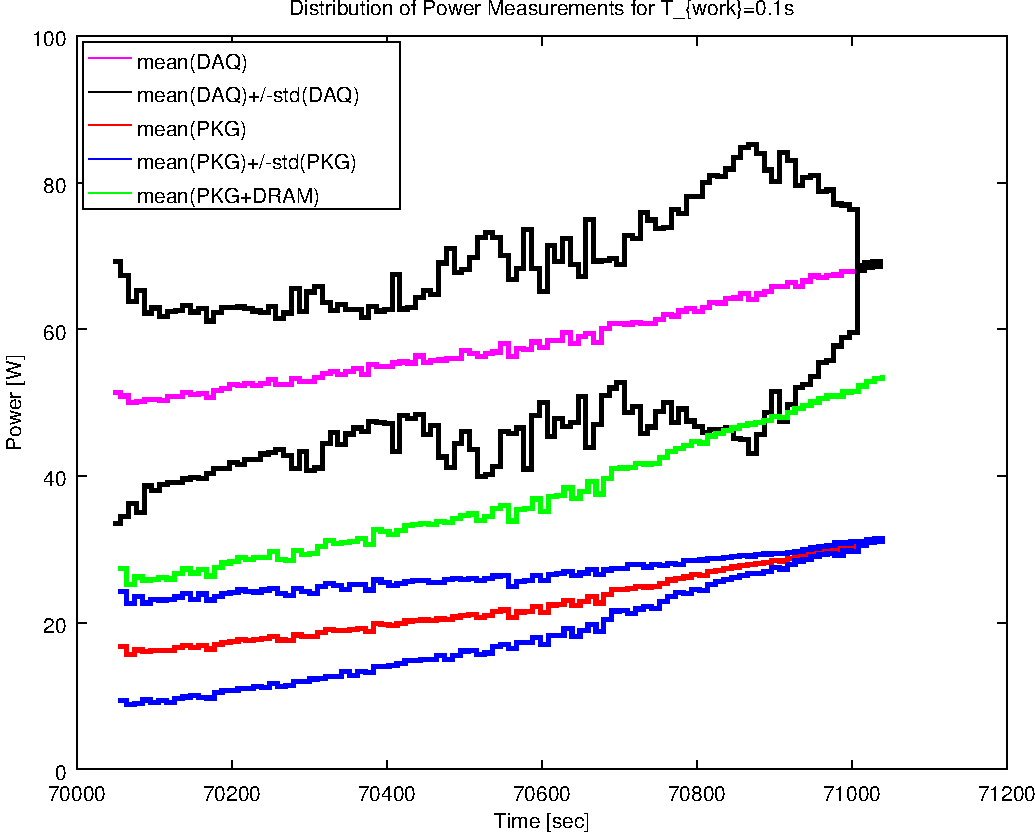
\includegraphics[width=\textwidth]{insertDelayTw100msCropped}
    \caption{Simulation Results}
    \label{simulationfigure}
\end{figure}

\section{Conclusion}
Write your conclusion here.

\end{document}
